% !TEX root = task-1-14-3.tex
% Editable task bank. Append new BankTask blocks at the end of the document.
\documentclass[12pt,a4paper]{article}
\usepackage{physics-textbook}
\usepackage{graphicx,needspace}
\usetikzlibrary{decorations.pathmorphing}
\newif\ifShowSolutions
\ifdefined\TutorEdition
  \ShowSolutionstrue
\else
  \ShowSolutionsfalse % Change to \ShowSolutionstrue to display solutions.
\fi
\newcounter{banktask}
\newsavebox{\BankTaskBox}
\newcommand{\BankTaskContent}[3]{%
  \noindent\textbf{\thebanktask.}\quad #2\par
  \ifShowSolutions
    \Needspace{50mm}% Keep the solution heading with its opening text or diagram.
    #3\par
    \ifdefined\TutorEdition
      \ifcsname TutorSource#1\endcsname
        \nopagebreak\smallskip{\small\csname TutorSource#1\endcsname\par}%
      \fi
    \fi
  \fi
}
\newcommand{\BankTask}[3]{%
  \refstepcounter{banktask}\par\medskip
  \sbox{\BankTaskBox}{\begin{minipage}{\linewidth}%
    \BankTaskContent{#1}{#2}{#3}\end{minipage}}%
  \ifdim\dimexpr\ht\BankTaskBox+\dp\BankTaskBox\relax>\dimexpr\textheight-20mm\relax
    \Needspace{35mm}\BankTaskContent{#1}{#2}{#3}%
  \else
    \Needspace{\dimexpr\ht\BankTaskBox+\dp\BankTaskBox\relax}%
    \noindent\usebox{\BankTaskBox}\par
  \fi
  \medskip
}
\begin{document}
\BookSubsection{1.14.3}{Импульс системы тел}


% Source sdamgia-402: https://phys-ege.sdamgia.ru/problem?id=402
\BankTask{sdamgia-402}{
Система состоит из двух тел $a$ и $b$. На рисунке стрелками в заданном масштабе указаны импульсы этих тел. Чему по модулю равен импульс всей системы? Округлите до десятых.


\begin{center}\begin{tikzpicture}[task graph]
\draw[gray!60,step=.45] (0,0) grid (2.25,3.6);
\draw[task curve] (.9,2.7)--(1.35,2.7) node[midway,above] {$2$ кг$\cdot$м/с};
\draw[task curve,->] (.45,1.35)--(.45,.45) node[right] {$\vec p_a$};
\draw[task curve,->] (1.8,1.8)--(.45,1.8) node[above] {$\vec p_b$};
\end{tikzpicture}\end{center}
}{
\smallskip\noindent\textbf{Решение}\par
Используя масштаб рисунка, определим модули импульсов тел $a$ и $b$. Из рисунка видно, что $|\vec p_a|=4\,\text{кг}\cdot\text{м/с}$ и $|\vec p_b|=6\,\text{кг}\cdot\text{м/с}.$ Импульс всей системы равен $\vec p_a+\vec p_b.$ Так как вектора $\vec p_a$ и $\vec p_b$ перпендикулярны, то модуль импульса всей системы равен:

$\sqrt{|\vec p_a|^2+|\vec p_b|^2}=\sqrt{4^2+6^2}\,\text{кг}\cdot\text{м/с}\approx7{,}2\,\text{кг}\cdot\text{м/с}.$

Ответ: $7{,}2$.
}

% Source sdamgia-403: https://phys-ege.sdamgia.ru/problem?id=403
\BankTask{sdamgia-403}{
Система состоит из двух тел $a$ и $b$. На рисунке стрелками в заданном масштабе указаны импульсы этих тел. Чему по модулю равен импульс всей системы?


\begin{center}\begin{tikzpicture}[task graph]
\draw[gray!60,step=.45] (0,0) grid (2.7,3.15);
\draw[task curve] (.9,2.25)--(1.35,2.25) node[midway,above] {$2$ кг$\cdot$м/с};
\draw[task curve,->] (1.35,.45)--(.45,1.35) node[above left] {$\vec p_b$};
\draw[task curve,->] (1.35,.45)--(2.25,1.35) node[above right] {$\vec p_a$};
\end{tikzpicture}\end{center}
}{
\smallskip\noindent\textbf{Решение}\par
\begin{center}\begin{tikzpicture}[task graph]
\draw[gray!60,step=.45] (0,0) grid (2.7,2.7);
\draw[task curve,->] (1.35,.45)--(.45,1.35) node[left] {$\vec p_b$};
\draw[task curve,->] (1.35,.45)--(2.25,1.35) node[right] {$\vec p_a$};
\draw[task curve,blue] (.45,1.35)--(1.35,2.25)--(2.25,1.35);
\draw[task curve,->,red] (1.35,.45)--(1.35,2.25);
\end{tikzpicture}\end{center}

Первый способ
Сложим импульсы по правилу параллелограмма, суммарный импульс обозначен на рисунке красной стрелкой. Видно, что его длина равна $4$ клеткам, следовательно, импульс системы по модулю равен $4\cdot2\,\text{кг}\cdot\text{м/с}=8\,\text{кг}\cdot\text{м/с}.$

Второй способ (более длинный и менее удачный)
Используя масштаб рисунка, определим модули импульсов тел $a$ и $b$. Из рисунка видно, что: 

$|\vec p_a|=|\vec p_b|=\sqrt{(4\,\text{кг}\cdot\text{м/с})^2+(4\,\text{кг}\cdot\text{м/с})^2}=4\sqrt2\,\text{кг}\cdot\text{м/с}.$

Импульс всей системы равен $\vec p_a+\vec p_b.$ Поскольку вектора $\vec p_a$ и $\vec p_b$ перпендикулярны, то модуль импульса всей системы равен: 

$\sqrt{|\vec p_a|^2+|\vec p_b|^2}=\sqrt{(4\sqrt2)^2+(4\sqrt2)^2}\,\text{кг}\cdot\text{м/с}=8\,\text{кг}\cdot\text{м/с}.$

Ответ: $8$.
}

% Source sdamgia-404: https://phys-ege.sdamgia.ru/problem?id=404
\BankTask{sdamgia-404}{
Система состоит из двух тел $1$ и $2$, массы которых равны $0{,}5\,\text{кг}$ и $2\,\text{кг}$. На рисунке стрелками в заданном масштабе указаны скорости этих тел. Чему равен импульс всей системы по модулю?


\begin{center}\begin{tikzpicture}[task graph]
\draw[gray!60,step=.45] (0,0) grid (1.8,3.15);
\draw[task curve] (.45,2.25)--(.9,2.25) node[midway,above] {$4$ м/с};
\fill (.9,.45) circle (1.4pt);\draw[task curve,->] (.9,.45)--(.9,1.8) node[left] {$\vec v_1$};
\draw[task curve,->] (.9,.45)--(1.35,.45) node[above right] {$\vec v_2$};
\end{tikzpicture}\end{center}
}{
\smallskip\noindent\textbf{Решение}\par
Используя масштаб рисунка, определим величины скоростей тел: $v_1=12\,\text{м/с}$ и $v_2=4\,\text{м/с}.$ Вычислим модули импульсов тел: 

$p_1=m_1v_1=0{,}5\,\text{кг}\cdot12\,\text{м/с}=6\,\text{кг}\cdot\text{м/с}$ и $p_2=m_2v_2=2\,\text{кг}\cdot4\,\text{м/с}=8\,\text{кг}\cdot\text{м/с}.$

Импульс всей системы равен $\vec p_1+\vec p_2.$ Поскольку вектора $\vec p_1$ и $\vec p_2$ перпендикулярны, то модуль импульса всей системы равен:

$\sqrt{|\vec p_1|^2+|\vec p_2|^2}=\sqrt{6^2+8^2}\,\text{кг}\cdot\text{м/с}=10\,\text{кг}\cdot\text{м/с}.$

Ответ: $10$.
}

% Source sdamgia-434: https://phys-ege.sdamgia.ru/problem?id=434
\BankTask{sdamgia-434}{
Перед столкновением два мяча движутся взаимно перпендикулярно, первый — с импульсом $p_1=3\,\text{кг}\cdot\text{м/с},$ а второй — с импульсом $p_2=4\,\text{кг}\cdot\text{м/с}.$ Чему равен модуль импульса системы мячей сразу после столкновения? Время столкновения считать малым, а столкновение — абсолютно упругим.
}{
\smallskip\noindent\textbf{Решение}\par
Для мячей выполняется закон сохранения импульсов. Импульс системы мячей сразу после столкновения равен полному импульсу системы до соударения. Таким образом, модуль импульса системы мячей равен:

$\sqrt{(3\,\text{кг}\cdot\text{м/с})^2+(4\,\text{кг}\cdot\text{м/с})^2}=5\,\text{кг}\cdot\text{м/с}.$

Ответ: $5$.
}

% Source sdamgia-7617: https://phys-ege.sdamgia.ru/problem?id=7617
\BankTask{sdamgia-7617}{
Тела $1$ и $2$ находятся на гладкой горизонтальной плоскости (см. рис., вид сверху). На них одновременно начинают действовать постоянные силы, равные соответственно $F_{1}=3\,\text{Н}$ и $F_{2}$. Чему равно изменение проекции импульса системы этих тел на ось $OX$ за первые две секунды?


\begin{center}\begin{tikzpicture}[task graph]
\draw[gray!60,step=.4] (0,0) grid (4,2.4);
\draw[task axis] (-.2,0)--(4.2,0) node[below] {$X$};\draw[task axis] (0,-.2)--(0,2.6) node[left] {$Y$};\node[below left] at (0,0) {$0$};
\fill (.4,1.6) circle (1.5pt) node[below] {$1$};\fill (3.6,.4) circle (1.5pt) node[below left] {$2$};
\draw[task curve,->] (.4,1.6)--(1.6,1.6) node[above] {$\vec F_1$};
\draw[task curve,->] (3.6,.4)--(2.4,2) node[above left] {$\vec F_2$};
\end{tikzpicture}\end{center}
}{
\smallskip\noindent\textbf{Решение}\par
Согласно второму закону Ньютона, сила есть отношение изменения импульса к промежутку времени, за которое произошло это изменение:

$F=\frac{\Delta p}{\Delta t}.$

Проекция силы $\vec F_1$ на ось $OX$ равна $3\,\text{Н}$, а значит, $\Delta p_1=F_1\Delta t=6\,\text{кг}\cdot\text{м/с}.$
Проекция силы $\vec F_2$ на ось $OX$ равна $-3\,\text{Н}$, а значит, $\Delta p_2=F_2\Delta t=-6\,\text{кг}\cdot\text{м/с}.$
Следовательно, изменение проекции импульса системы этих тел на ось $OX$ равно $0$.

Ответ: $0$.
}

% Source sdamgia-19688: https://phys-ege.sdamgia.ru/problem?id=19688
\BankTask{sdamgia-19688}{
Два шарика — стальной, массой $m_{1}=50\,\text{г}$, и пластилиновый, массой $m_{2}=200\,\text{г}$ — начинают двигаться по гладкой горизонтальной плоскости вдоль одной прямой по направлению к закрепленной стенке (см. рис.). Скорости шариков одинаковы по модулю и равны $2\,\text{м/с}$. Линия движения шариков перпендикулярна стенке. Стальной шарик сталкивается со стенкой абсолютно упруго, а пластилиновый — абсолютно неупруго. Определите модуль полного импульса, который был передан стенке шариками в результате соударения с ней. 


\begin{center}\begin{tikzpicture}[task graph]
\draw[task curve] (0,0)--(4,0);\foreach \x in {0,.2,...,4}{\draw (\x,0)--++(-.12,-.12);}
\draw[fill=orange!25] (2,0) rectangle (2.1,1.1);
\draw[fill=orange!25] (.6,.15) circle (.13) node[above=3pt] {$m_2$};\draw[task curve,->] (.75,.15)--(1.3,.15);
\draw[fill=orange!25] (3.4,.15) circle (.13) node[above=3pt] {$m_1$};\draw[task curve,->] (3.25,.15)--(2.7,.15);
\end{tikzpicture}\end{center}
}{
\smallskip\noindent\textbf{Решение}\par
\begin{center}\begin{tikzpicture}[task graph]
\draw[task axis] (0,0)--(5,0) node[below] {$x$};
\foreach \x in {1.5,3.5}{\draw[fill=orange!25] (\x,.4) rectangle ++(.08,1.3);}
\draw[fill=orange!25] (.4,1) circle (.1);\draw[task curve,->] (.6,1)--(1.1,1) node[above] {$\vec v_{02}$};
\draw[fill=orange!25] (4.8,1.4) circle (.1);\draw[task curve,->] (4.6,1.4)--(4,1.4) node[above] {$\vec v_{01}$};
\draw[fill=orange!25] (4,.5) circle (.1);\draw[task curve,->] (4.2,.5)--(4.9,.5) node[above] {$\vec v_1$};
\end{tikzpicture}\end{center}

При абсолютно упругом ударе $v_{01}=v_1=v.$ Изменение импульса стального шарика равно $\Delta\vec p_1=m_1\vec v_1-m_1\vec v_{01},$ $\Delta p_{1x}=m_1v_1+m_1v_{01}=2m_1v.$ При абсолютно неупругом ударе $v_2=0.$ Изменение импульса пластилинового шарика равно $\Delta\vec p_2=m_2\vec v_2-m_2\vec v_{02},$ $\Delta p_{2x}=-m_2v_{02}=-m_2v.$ Импульс, переданный стенке, равен

$p_x=\Delta p_{1x}+\Delta p_{2x}=2m_1v-m_2v=v(2m_1-m_2),$
$|p_x|=v|2m_1-m_2|=2\cdot|2\cdot0{,}05-0{,}2|=0{,}2\,\text{кг}\cdot\text{м/с}.$

Ответ: $0{,}2$.
}

% Source sdamgia-6483: https://phys-ege.sdamgia.ru/problem?id=6483
\BankTask{sdamgia-6483}{
На неподвижный бильярдный шар налетел другой такой же шар. Налетевший шар имел до удара импульс $p=0{,}5\,\text{кг}\cdot\text{м/с}$. После удара шары разлетелись под углом $90^\circ$ так, что импульс одного $p_{1}=0{,}4\,\text{кг}\cdot\text{м/с}$ (см. рисунок). Каков импульс другого шара после соударения?


\begin{center}\begin{tikzpicture}[task graph]
\draw[fill=orange!25] (0,0) circle (.13);\draw[task curve,->] (.15,0)--(.85,0) node[above] {$\vec p$};
\draw (1.1,0) circle (.13);\draw[fill=orange!25] (1.5,.7) circle (.13);\draw[fill=orange!25] (1.8,-.4) circle (.13);
\draw[task curve,->] (1.65,.95)--(1.95,1.5) node[left] {$\vec p_2$};\draw[task curve,->] (2,-.52)--(2.7,-.92) node[below] {$\vec p_1$};
\draw (1.2,.18)--(1.38,.08)--(1.28,-.1);
\end{tikzpicture}\end{center}
}{
\smallskip\noindent\textbf{Решение}\par
\begin{center}\begin{tikzpicture}[task graph]
\draw[task curve,->] (0,0)--(.9,1.5) node[left] {$\vec p_2$};
\draw[task curve,->] (.9,1.5)--(3.4,0) node[above right] {$\vec p_1$};
\draw[task curve,->] (0,0)--(3.4,0) node[below] {$\vec p$};\draw (.8,1.33)--(.98,1.23)--(1.08,1.41);
\end{tikzpicture}\end{center}

По закону сохранения импульса импульс системы до соударения шаров и после должен быть одинаков: $\vec p=\vec p_1+\vec p_2.$
Построим сумму векторов $\vec p_1$ и $\vec p_2,$ (см. рис.) получим прямоугольный треугольник. Найдем импульс второго шара из теоремы Пифагора:

$p_2=\sqrt{p^2-p_1^2}=\sqrt{(0{,}5\,\text{кг}\cdot\text{м/с})^2-(0{,}4\,\text{кг}\cdot\text{м/с})^2}=0{,}3\,\text{кг}\cdot\text{м/с}.$

Ответ: $0{,}3$.
}

% Source sdamgia-3313: https://phys-ege.sdamgia.ru/problem?id=3313
\BankTask{sdamgia-3313}{
Папа, обучая девочку кататься на коньках, скользит с ней по льду со скоростью $4\,\text{м/с}$. В некоторый момент он аккуратно толкает девочку в направлении движения. Скорость девочки при этом возрастает до $6\,\text{м/с}$. Масса девочки $20\,\text{кг}$, а папы $80\,\text{кг}$. Какова скорость папы после толчка? Трение коньков о лед не учитывайте.
}{
\smallskip\noindent\textbf{Решение}\par
Поскольку на систему в горизонтальном направлении не действует никаких внешних сил, для системы папа+девочка выполняется закон сохранения импульса в этом направлении: $(m_{\text{д}}+m_{\text{п}})v=m_{\text{д}}v_2+m_{\text{п}}u.$
Решая это уравнение, находим скорость папы после толчка: 

$u=\frac{(m_{\text{д}}+m_{\text{п}})v-m_{\text{д}}v_2}{m_{\text{п}}}=\frac{(20+80)\cdot4-20\cdot6}{80}=3{,}5\,\text{м/с}.$

Ответ: $3{,}5\,\text{м/с}$.
}

% Source sdamgia-29741: https://phys-ege.sdamgia.ru/problem?id=29741
\BankTask{sdamgia-29741}{
Тележка массой $50\,\text{кг}$ и скорость $1\,\text{м/с}$ движется вправо по гладкой дороге. Мальчик массой $50\,\text{кг}$ прыгает навстречу тележке со скоростью $2\,\text{м/с}$. Найти модуль скорости тележки с мальчиком после прыжка мальчика.
}{
\smallskip\noindent\textbf{Решение}\par
Учитывая, что импульс тележки до взаимодействия меньше импульса мальчика, делаем вывод, что после прыжка мальчика тележка поедет в противоположную сторону. Изобразим скорости тел до и после взаимодействия (см. левый и правый рисунок).

\begin{center}\begin{tikzpicture}[task graph]
\draw[fill=orange!25] (0,0) rectangle (.7,.45);\node[below] at (.35,0) {$m_1$};\draw[task curve,->] (.7,.22)--(1.5,.22) node[above] {$\vec v_1$};
\draw[fill=orange!25] (2.8,0) rectangle (2.95,.65);\node[below] at (2.87,0) {$m_2$};\draw[task curve,->] (2.8,.22)--(2,.22) node[above] {$\vec v_2$};
\begin{scope}[xshift=4cm]
\draw[fill=orange!25] (1,0) rectangle (1.7,.45);\draw[fill=orange!25] (1,.45) rectangle (1.15,1);\node[below] at (1.3,0) {$m_1+m_2$};\draw[task curve,->] (1,.45)--(0,.45) node[above] {$\vec u$};
\end{scope}\end{tikzpicture}\end{center}


Так как поверхность гладкая, то система тел замкнутая, можно применить закон сохранения импульса: 

$m_1\vec v_1+m_2\vec v_2=(m_1+m_2)\vec u.$

Выберем ось, направив ее влево. В проекции на эту ось: 

$m_2v_2-m_1v_1=(m_1+m_2)u.$

Отсюда скорость тележки после взаимодействия: 

$u=\frac{m_2v_2-m_1v_1}{m_1+m_2}=\frac{50\cdot2-50\cdot1}{50+50}=0{,}5\,\text{м/с}.$

Ответ: $0{,}5\,\text{м/с}$.
}

% Source sdamgia-19875: https://phys-ege.sdamgia.ru/problem?id=19875
\BankTask{sdamgia-19875}{
Два пластилиновых шарика массами $m$ и $3m$ летят навстречу друг другу с одинаковыми по модулю скоростями. После абсолютно неупругого удара их скорость стала равна $0{,}5\,\text{м/с}$. Найдите первоначальную скорость.
}{
\smallskip\noindent\textbf{Решение}\par
\begin{center}\begin{tikzpicture}[task graph]
\draw[task axis] (0,0)--(4,0) node[below] {$x$};\draw[task axis] (0,-1.6)--(4,-1.6) node[below] {$x$};
\draw[fill=orange!25] (.7,.8) circle (.3) node[above=8pt] {$3m$};\draw[task curve,->] (1,.8)--(1.7,.8) node[above] {$\vec V$};
\draw[fill=orange!25] (3.2,.6) circle (.2) node[above=6pt] {$m$};\draw[task curve,->] (3,.6)--(2.3,.6) node[above] {$\vec V$};
\draw[fill=orange!25] (1.1,-.85) circle (.3) node[left=8pt] {$3m$};\draw[fill=orange!25] (1.6,-1) circle (.2) node[below=6pt] {$m$};\draw[task curve,->] (1.7,-.85)--(2.6,-.85) node[above] {$\vec V_1$};
\end{tikzpicture}\end{center}

По закону сохранения импульса: $\vec p_1+\vec p_2=\vec p_0.$ 
Проекция на ось $x$: $3mv-mv=4mv_1;$ $2mv=4mv_1.$ 
Откуда первоначальная скорость шаров равна

$v=2v_1=2\cdot0{,}5=1\,\text{м/с}.$

Ответ: $v=1\,\text{м/с}.$
}


% Source DC8C1F: https://ege.fipi.ru/bank/questions.php?search=1&proj=BA1F39653304A5B041B656915DC36B38&qid=DC8C1F
\BankTask{DC8C1F}{
Два тела движутся по взаимно перпендикулярным пересекающимся прямым, как показано на рисунке. Модуль импульса первого тела $p_1=8\,\text{кг}\cdot\text{м}/\text{с}$, второго тела $p_2=6\,\text{кг}\cdot\text{м}/\text{с}$. Каков модуль импульса системы этих тел после их абсолютно неупругого удара? Выразите ответ в $\text{кг}\cdot\text{м}/\text{с}$.
\begin{center}
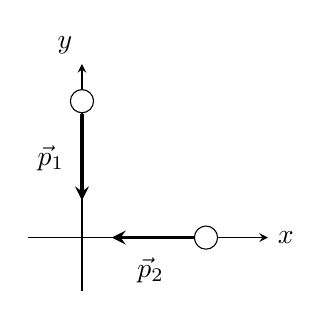
\begin{tikzpicture}[>=stealth,scale=1.05]
\draw[->] (-0.65,0)--(2.25,0) node[right] {$x$};
\draw[->] (0,-0.65)--(0,2.1) node[above left] {$y$};
\draw[fill=white] (0,1.65) circle (0.14);
\draw[very thick,->] (0,1.49)--(0,0.45);
\node[left] at (-0.1,0.96) {$\vec p_1$};
\draw[fill=white] (1.5,0) circle (0.14);
\draw[very thick,->] (1.35,0)--(0.36,0);
\node[below] at (0.83,-0.12) {$\vec p_2$};
\end{tikzpicture}
\end{center}
}{
\smallskip\noindent\textbf{Решение от GPT}\par
Импульс системы сохраняется. До удара импульсы перпендикулярны, поэтому $p=\sqrt{p_1^2+p_2^2}=\sqrt{8^2+6^2}=10\,\text{кг}\cdot\text{м}/\text{с}$. Ответ: $10\,\text{кг}\cdot\text{м}/\text{с}$.
}

\end{document}
